\documentclass{beamer}
\usetheme{metropolis}

\usepackage{tikz}

\usepackage{tikz}
\usepackage{animate}
\usepackage{ifthen}

\usepackage[T1]{fontenc}
\usepackage[utf8]{inputenc}

\usepackage{graphicx}
\graphicspath{ {./} }

\usepackage{listings}

\lstset{basicstyle=\ttfamily\footnotesize}

\makeatletter
\def\verbatim@font{\footnotesize\ttfamily}
\makeatother

\title{Laserowy kotek}
\subtitle{gra roku 2023 i pół}
\author{Weronika Jakimowicz}
\date{Styczeń 2024}


\begin{document}

\begin{frame}
  \maketitle 
  \begin{tikzpicture}[overlay, remember picture]
    \node at (9,8) {
\includegraphics[width=0.3\textwidth]{tytul_obrazek.jpg}};
  \end{tikzpicture}
\end{frame}

\section{Jaki jest plan?}

\begin{frame}
  \frametitle{$k$-szkielet gry}

  \begin{itemize}
    \item Gracz jest Kycią, unika Czarnego Psa
    \item Czarny Pies pojawia się z prawej strony ekranu i leci w lewo

  \item Lepsza grafika niż na załączonym obrazku

  \begin{center}
    \animategraphics[autoplay,loop]{10}{anim0}{1}{8}
  \end{center}

    \item Mało stresu i próba robienia gry bez Unity
  \end{itemize}

  
\end{frame}

\section{Narzędzia}

\begin{frame}
  \frametitle{Wielbłąd juczny}

  \begin{itemize}
    \item Kochany język obiektowy \lstinline{Ocaml}
    \item Biblioteka \lstinline{raylib} wraz z \lstinline{ragui}

    \scalebox{0.6}{\lstinline{raylib}: \url{https://www.raylib.com/}}

    \scalebox{0.6}{\lstinline{raylib} dla 
\includegraphics[width=4mm]{ocaml.png}: \url{https://github.com/tjammer/raylib-ocaml} }
  
  \item Dune?

      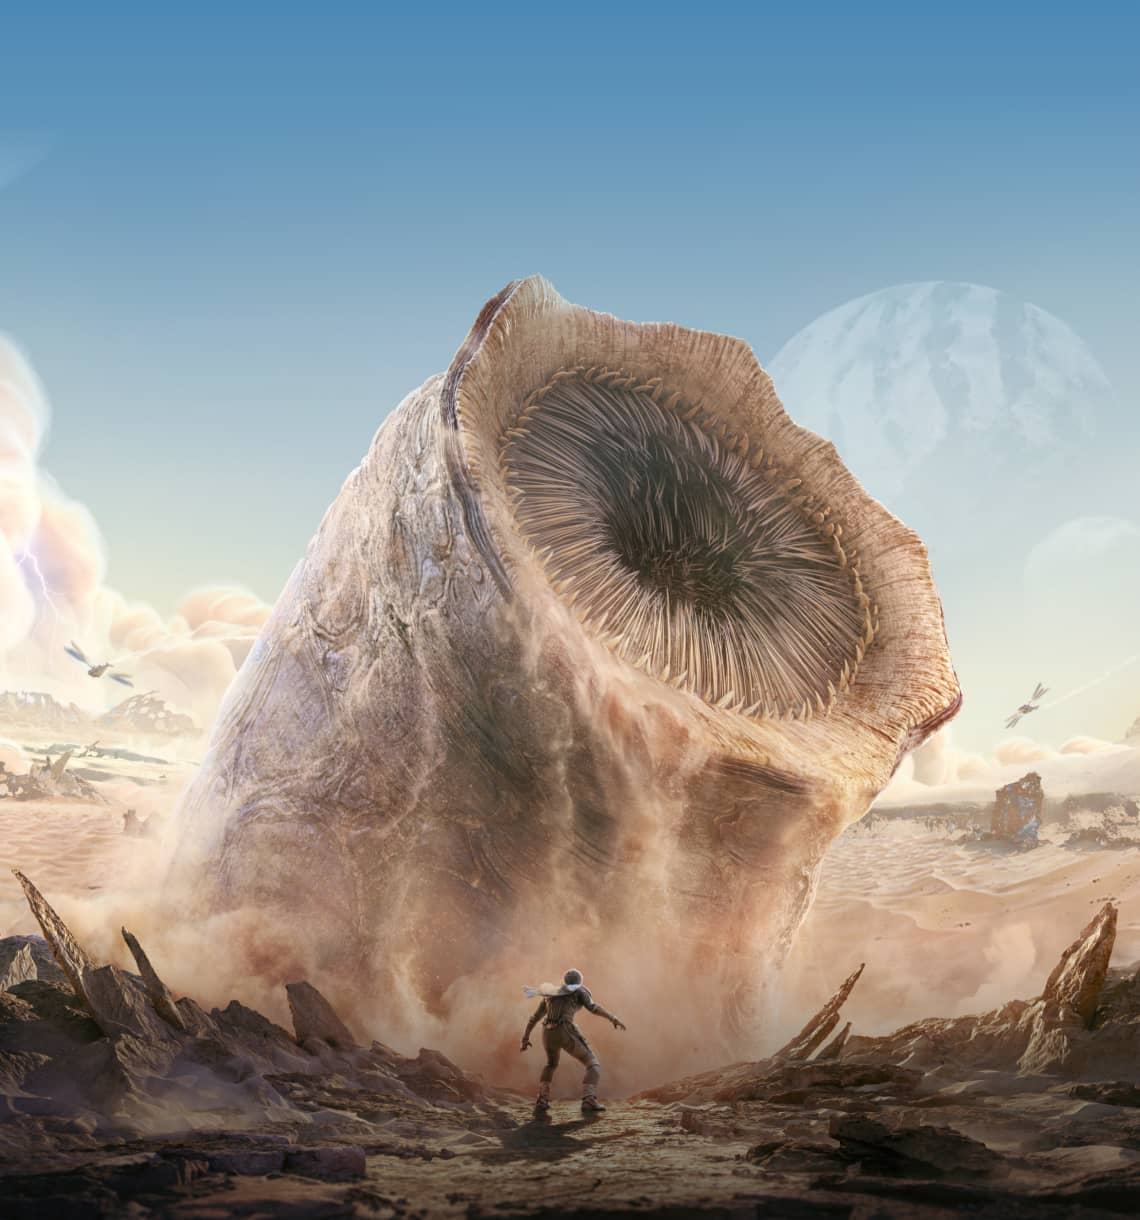
\includegraphics[height=3cm]{./dune.jpg}
  \end{itemize}
\end{frame}

\section{Troszkę o kodzie}

\begin{frame}
  \begin{itemize}
    \item Typy zamiast obiektów - gracz, przeciwnik, tło etc. dostają własny typ będący rekordem
    \item Typy zamiast boolów
    \item Leniwość tylko w designie, nie w kodzie!
  \end{itemize}
\end{frame}

\begin{frame}
  \section{Koniec!}

  \begin{tikzpicture}[overlay, remember picture]
    \node at (8, 0) {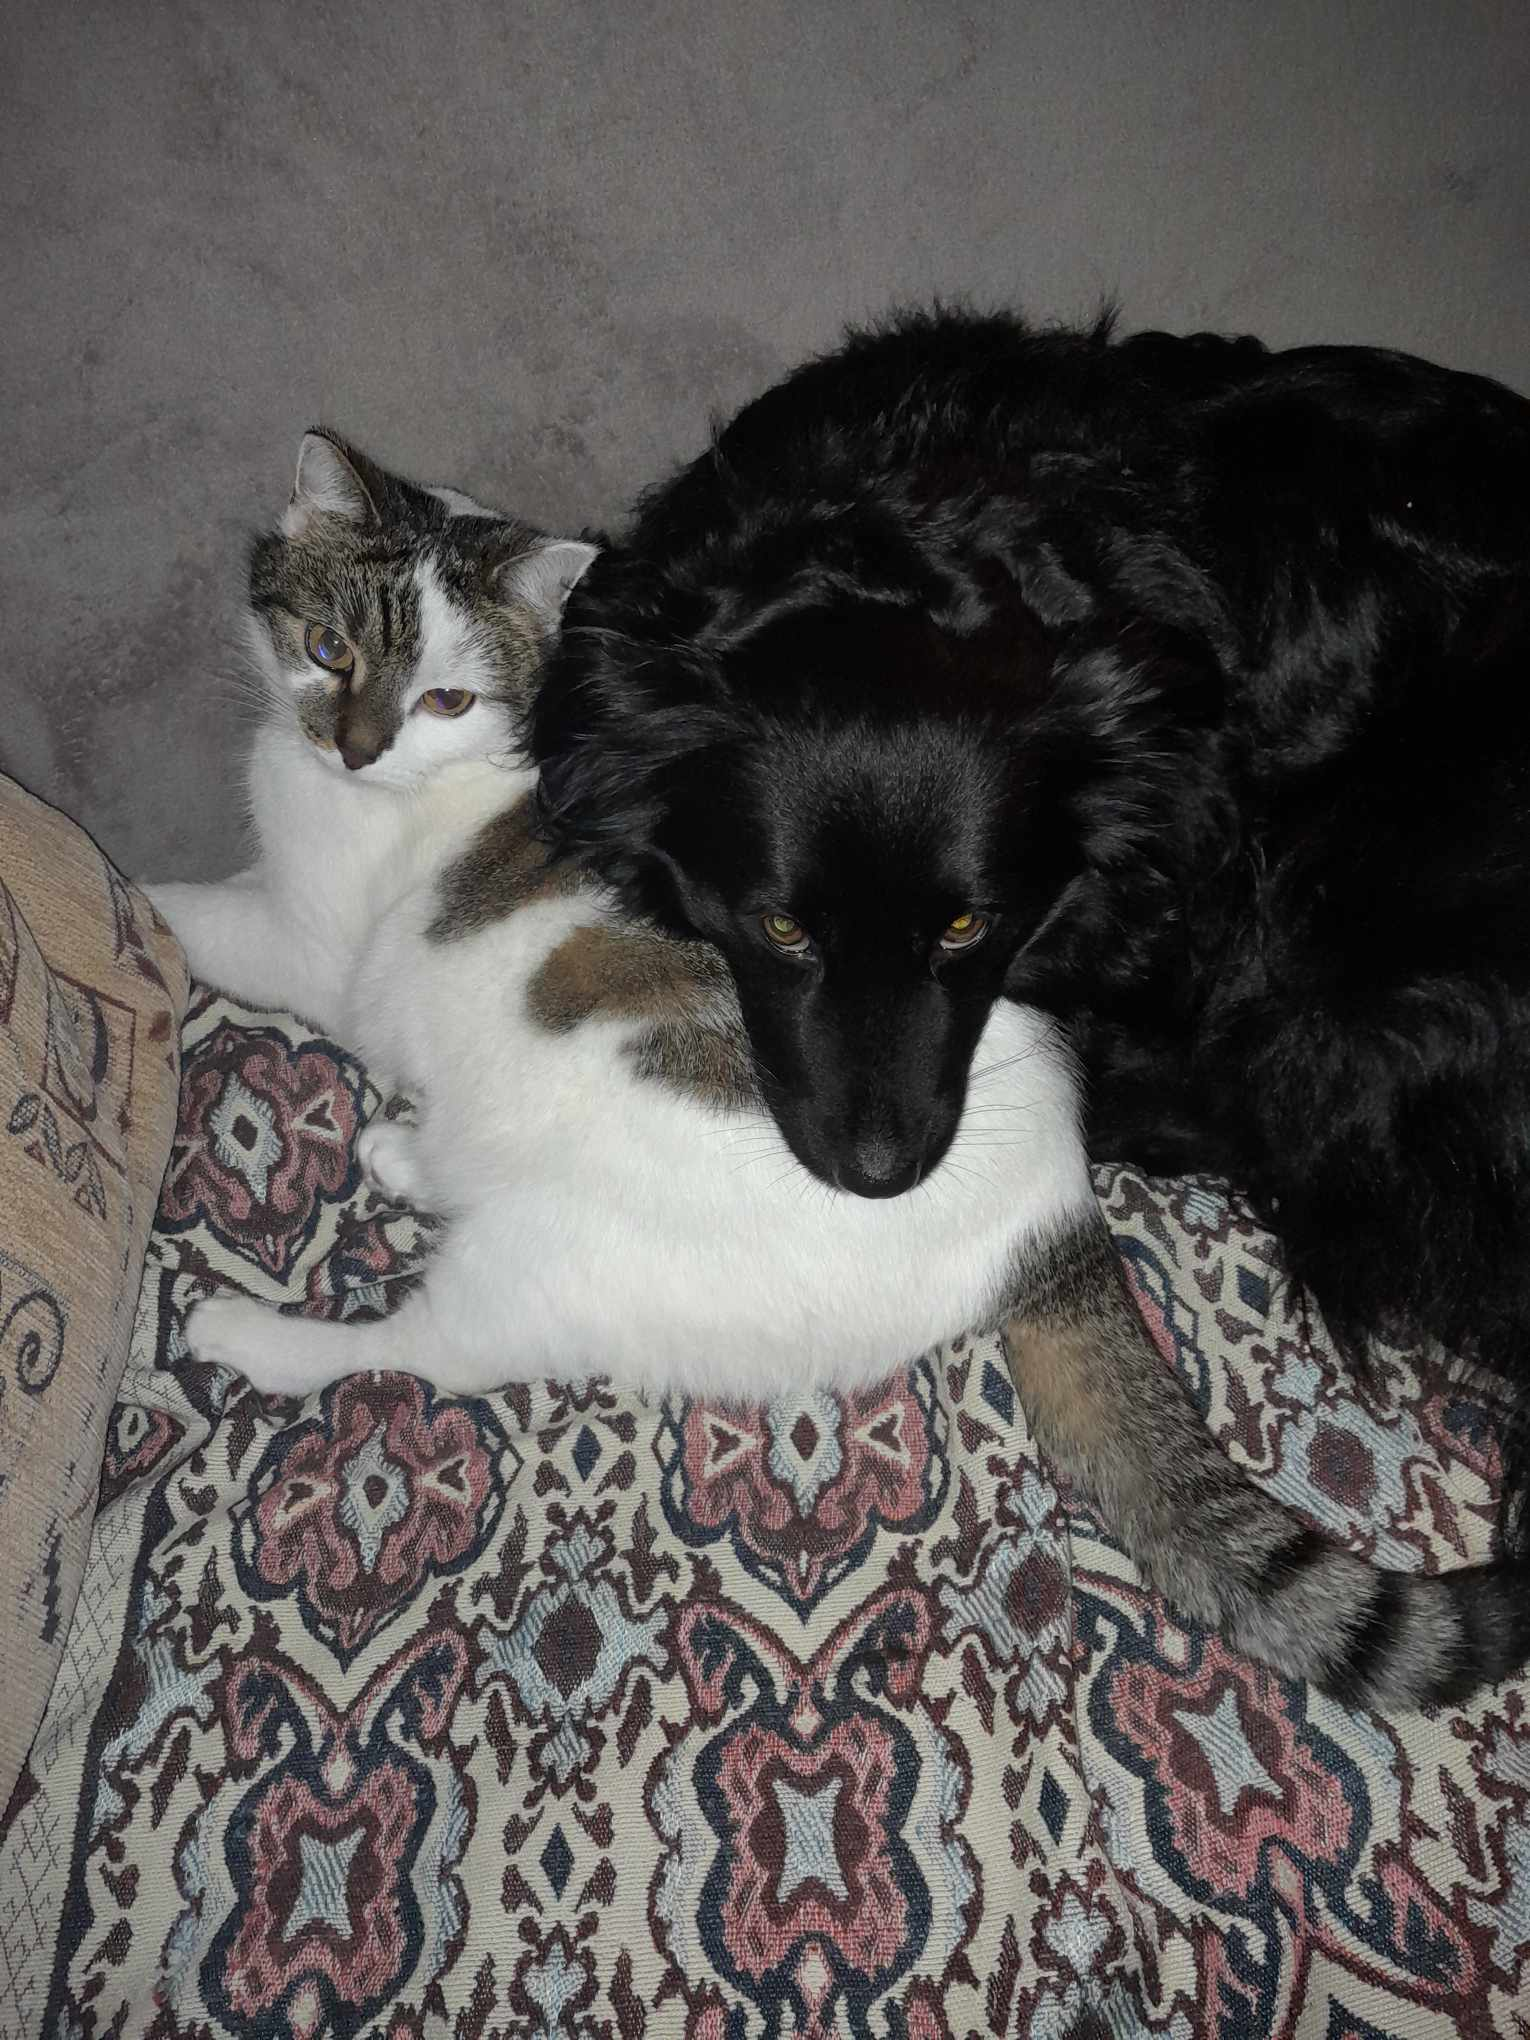
\includegraphics[height=0.8\textheight]{zwierzyniec.jpg}};
  \end{tikzpicture}
\end{frame}

\end{document}
